\chapter{prior modelling}

\begin{figure}[ht!]
	\centering
	\input{TruePress.pdf_tex}
	\caption[]{}
	\label{fig:TruePressFunc}
\end{figure}


\begin{figure}[ht!]
	\centering
	\input{TrueTemp.pdf_tex}
	\caption[]{}
	\label{fig:TrueTempFunc}
\end{figure}

\begin{figure}[ht!]
	\centering
	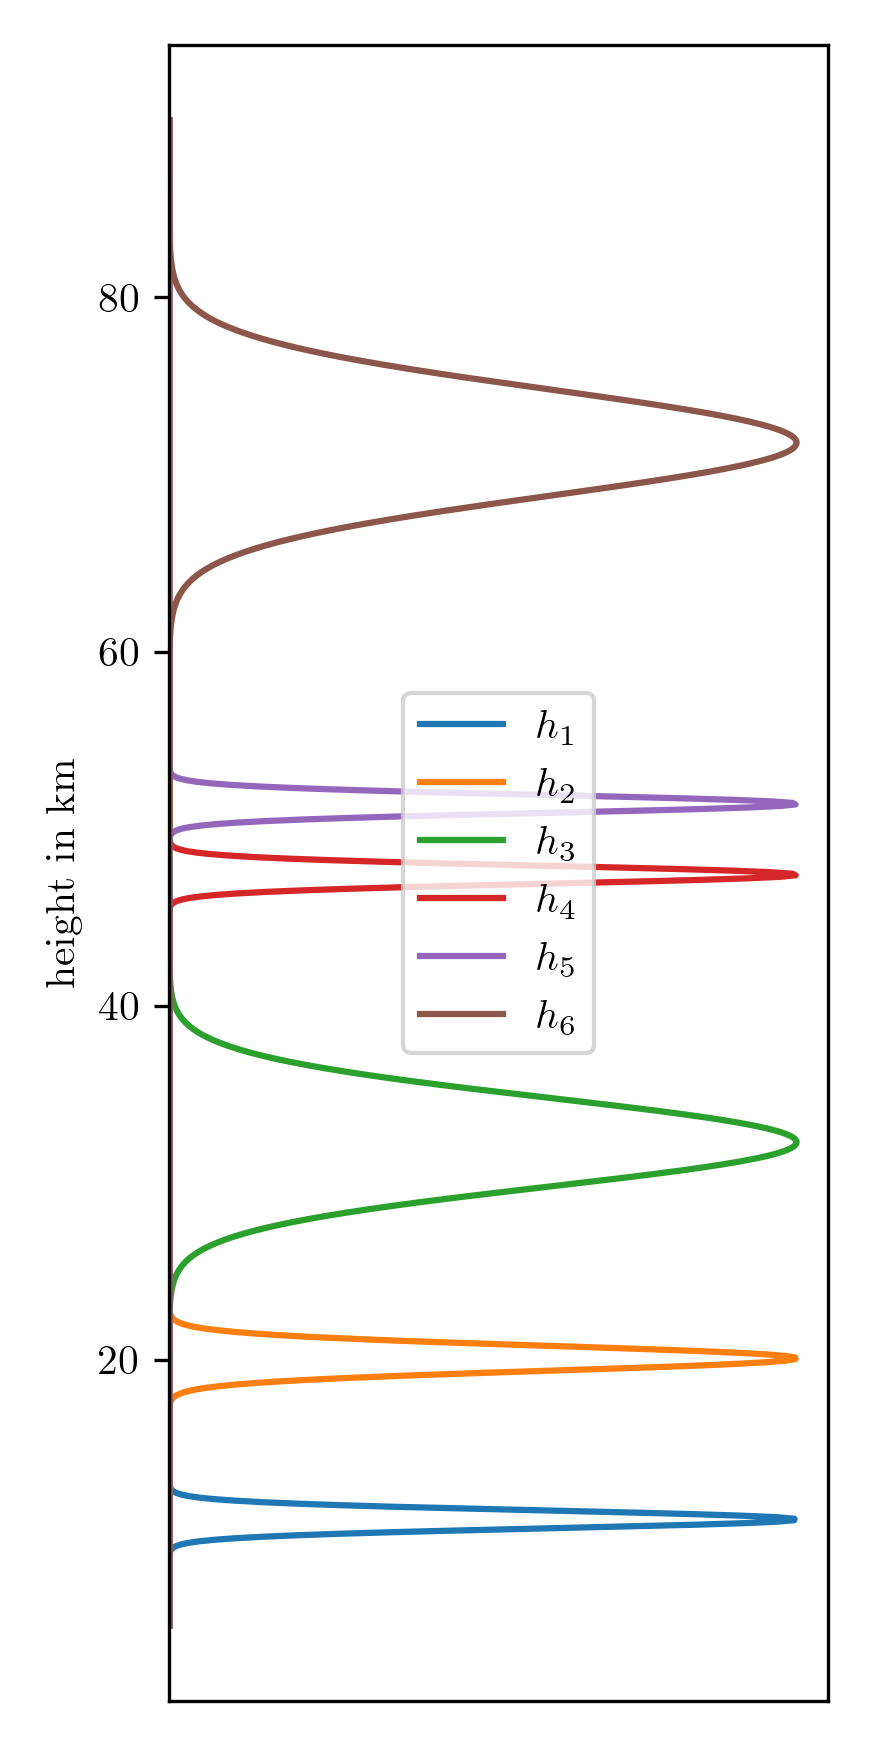
\includegraphics{HeightPriors.png}
	\caption[]{}
	\label{fig:HeightPriors}
\end{figure}




\begin{figure}[ht!]
	\centering
	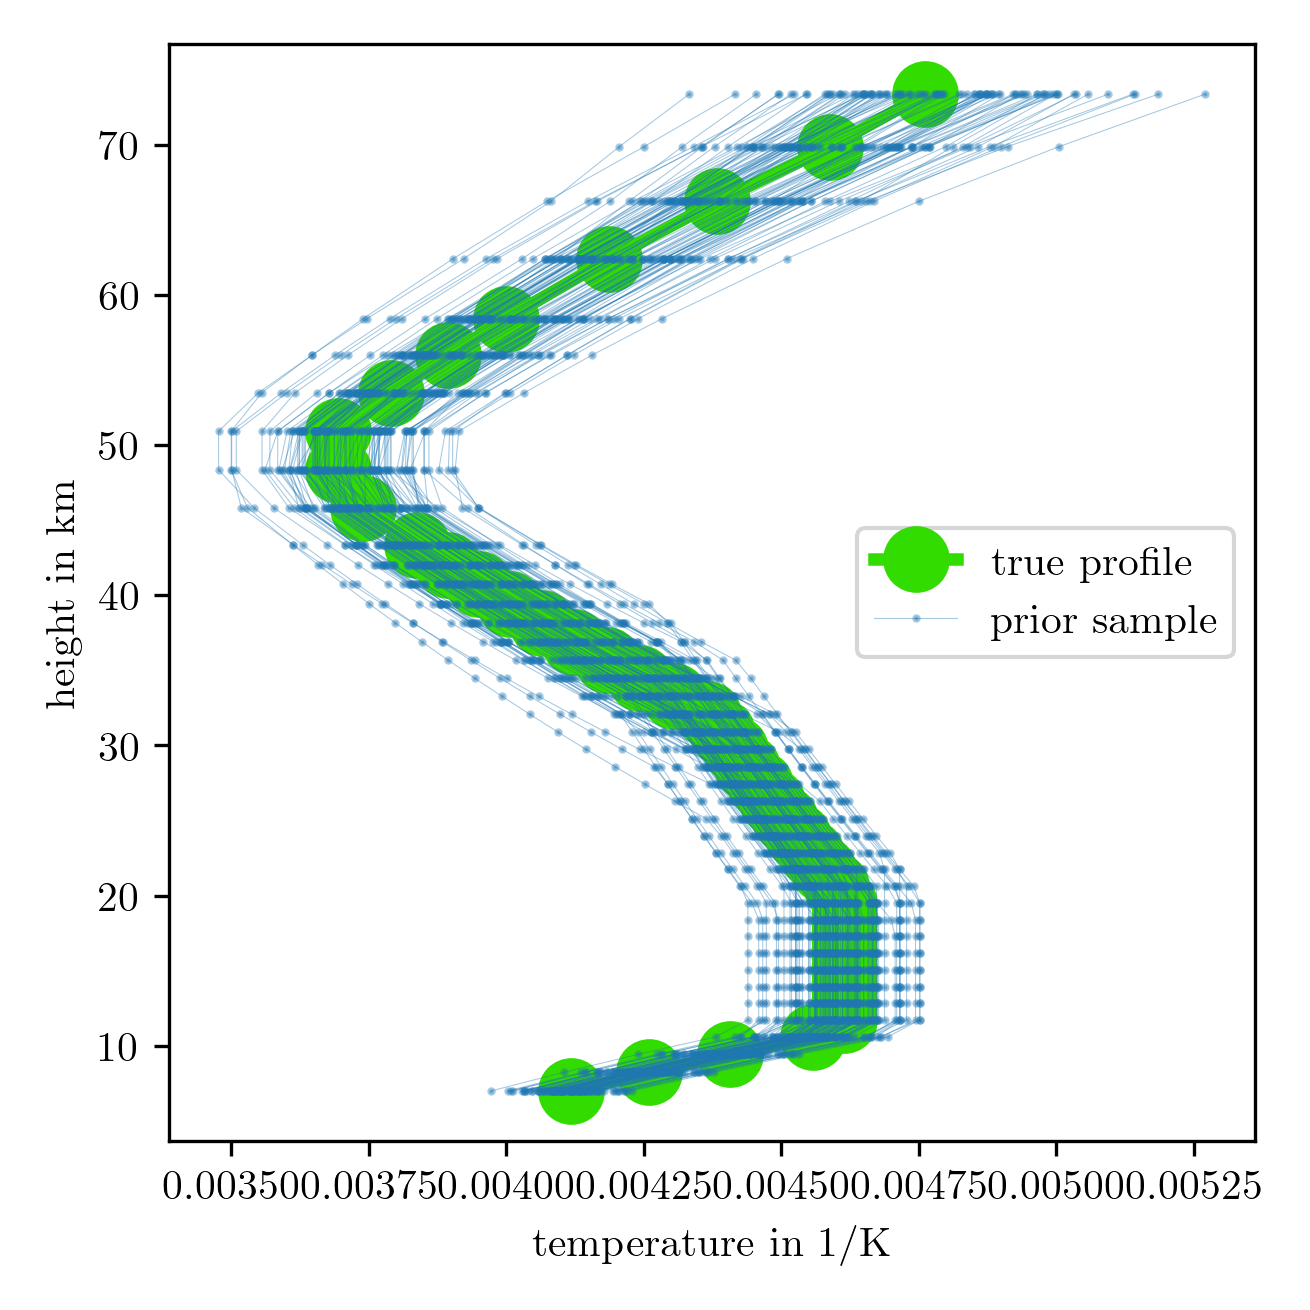
\includegraphics{PriorOverTempPost.png}
	\caption[]{}
	\label{fig:OverTempPrior}
\end{figure}

\begin{figure}[ht!]
	\centering
	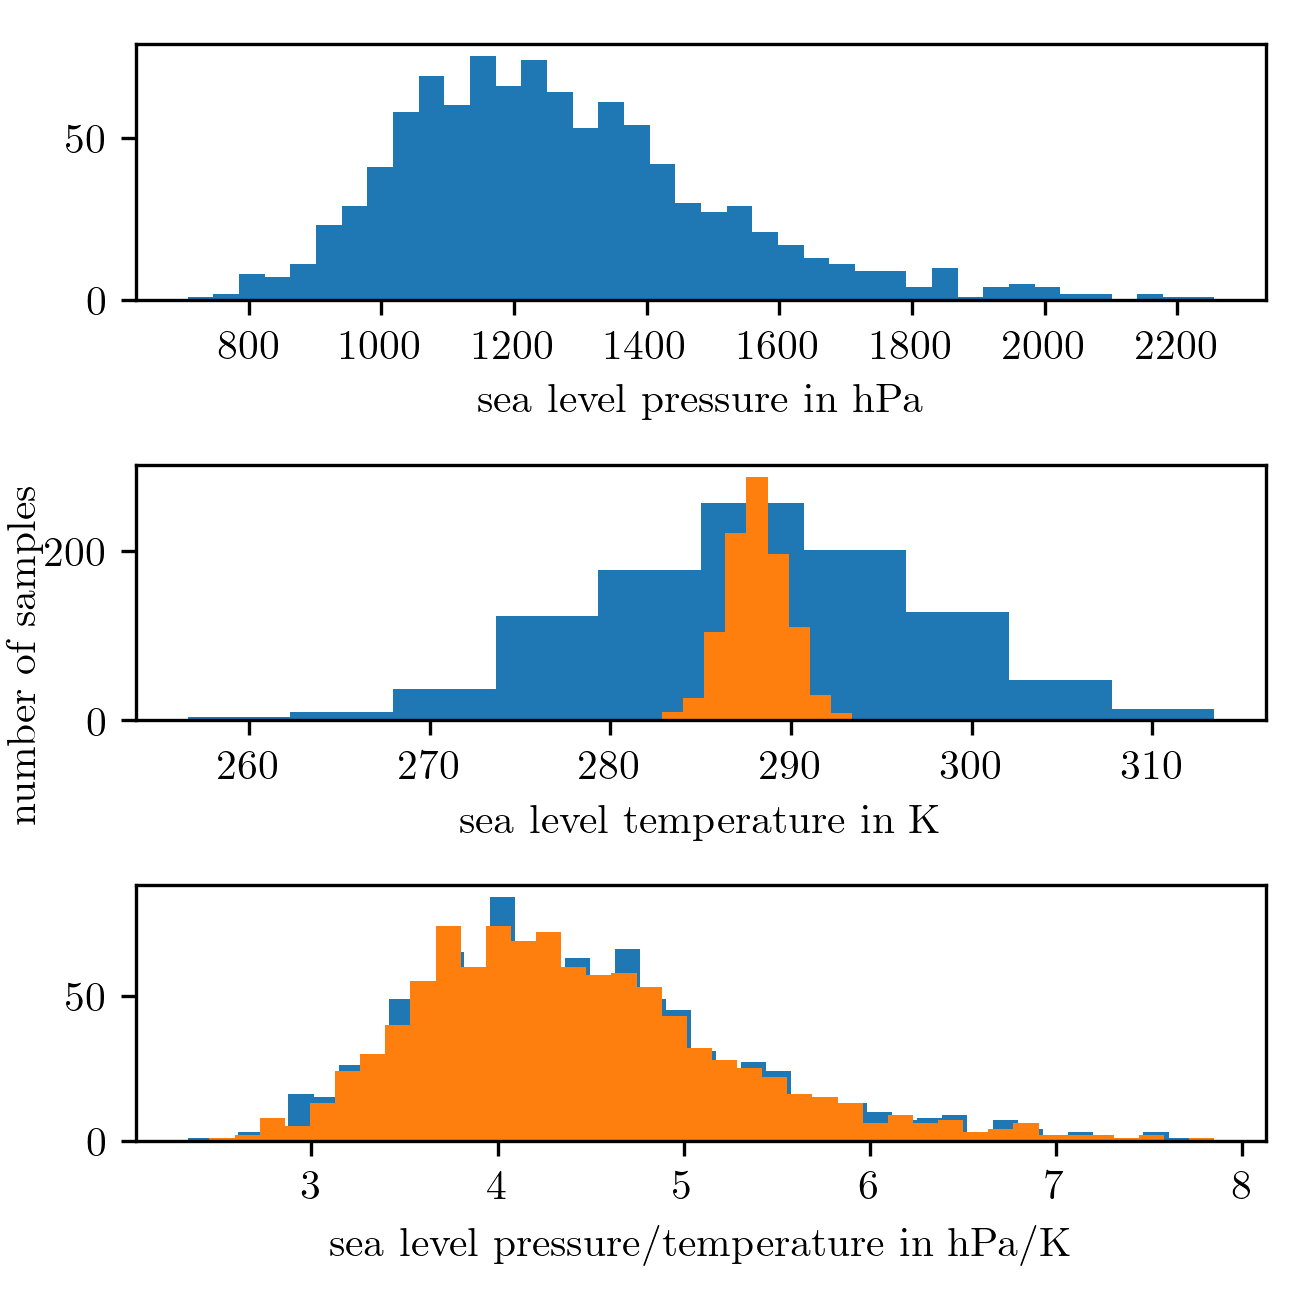
\includegraphics{SeaLevelHist.png}
	\caption[]{}
	\label{fig:SeaLevelHist}
\end{figure}

\section{t-walk}

\begin{figure}[ht!]
	\centering
	\includegraphics{TraceTwalk.png}
	\caption[]{}
	\label{fig:TraceTwalk}
\end{figure}
